\chapter{绪论}
%
\section{研究背景和意义}
%
垂直领域检索增强对话生成任务有助于提高用户体验、解决特定领域的问题和提供个性化的服务。它可以应用于医疗保健、金融、法律、教育、科技等领域,为用户提供更加专业、全面和个性化的信息交流和服务。因此,垂直领域检索增强对话生成任务对于满足用户需求、提高工作效率、提供个性化服务等方面具有重要意义。

垂直领域检索增强对话生成目前主要的挑战是领域知识丰富,用户问题多种多样且抽象。针对领域知识丰富的挑战,研究人员致力于构建更加智能和灵活的对话生成模型,能够充分利用领域内的丰富知识资源,包括专业词汇、行业规范、学术研究成果等,以更好地应对用户的专业性问题。这包括基于知识图谱和预训练语言模型的技术,以及定制化的领域知识处理方法。针对用户问题多样性和抽象性的挑战,研究人员在探索如何构建更加灵活和多样化的对话生成模型,能够理解和回答各种类型的问题,包括事实性问题、推理性问题、情绪化问题\cite{JSJX202312001}等。此外,研究人员也致力于开发更加智能、个性化的对话交互方式,以满足用户多样化的沟通需求。同时,深度学习技术在对话生成任务中的应用也在不断演进。例如,针对领域知识丰富和用户问题多样性的挑战,研究人员正在探索如何通过多模态融合(如文本、图像、语音)、增强学习、迁移学习等技术手段,提高对话生成模型的适应性和泛化能力。

然而,相对于开放域对话生成,垂直领域对话内容更复杂、背景知识要求更多,生成准确、真实、可靠回复的技术挑战性更高,使垂直领域检索增强对话生成存在以下几个难点:

\begin{itemize}[topsep = 0 pt, itemsep= 0 pt, parsep=0pt, partopsep=0pt, leftmargin=36pt, itemindent=0pt, labelsep=6pt, listparindent=24pt]
	\item 难点1:垂直领域背景知识丰富,且逻辑相对复杂。
	\item 难点2:用户问题形式多样,且意图难以理解。
\end{itemize}

近年来,越来越多研究人员投身面向垂直领域的检索增强对话生成研究\cite{RJXB202402009}。来自斯坦福大学、加利福尼亚大学、清华大学等国内外高校和企业研究机构的学者在该领域开展了大量研究工作。国际上的一些主流学术会议和学术期刊也将垂直领域检索增强对话生成作为一个研究热点,如ACL、EMNLP等国际会议。综上,面向垂直领域的检索增强对话生成研究是当前人工智能领域的重点与热点,不仅具有重要的理论价值,而且具有丰富的实际应用价值。

\section{本文主要研究内容}

如前所述,面向垂直领域的检索增强对话生成的关键在于解决以下挑战:1)垂直领域背景知识丰富,且逻辑相对复杂;2)用户问题形式多样,且意图难以理解。

\begin{figure}[htbp]
	\centering
	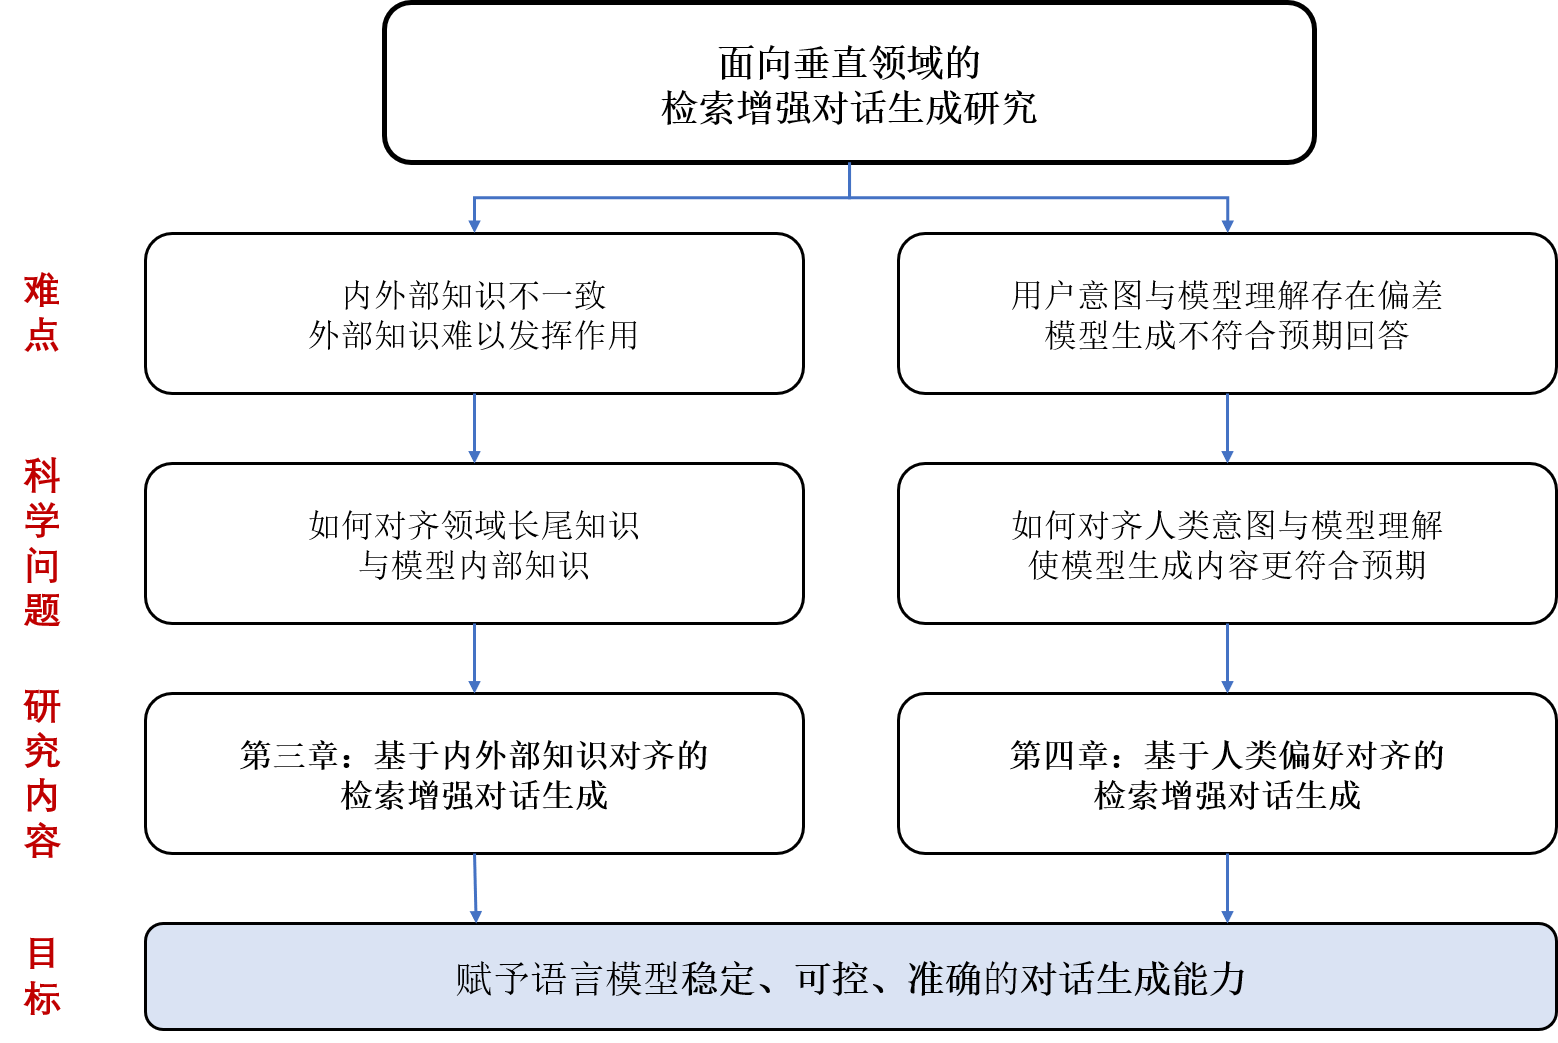
\includegraphics[scale=0.55]{Fig/paper_structure.png}
	\caption{\label{research_idea_and_research_content_of_this_paper}本文的研究思路与研究内容。}
\end{figure}

为解决上述挑战,本文进行了两个方面的研究,研究思路与研究内容如图1-1所示。包括基于内外部知识对齐的垂直领域对话生成和基于人类偏好的对话生成对齐。具体研究内容如下:

\begin{enumerate}[topsep = 0 pt, itemsep= 0 pt, parsep=0pt, partopsep=0pt, leftmargin=0pt, itemindent=44pt, labelsep=6pt, listparindent=24pt, label=\arabic*)]
	\item 基于内外部知识对齐的检索增强对话生成
	
	大模型在预训练中没见过垂直领域的长尾知识,因此检索增强所补充的知识文档可能未能与模型内部知识完全对齐。为此,本文对内外部知识的对齐展开研究,利用一个语义切分模块提取知识文档的文档级信息和实体级信息,并将提取出来的知识分别用于构建外部知识库和内部知识注入,实现垂直领域对话模型内外部知识对齐。

	\item 基于人类偏好对齐的检索增强对话生成
	
	弥合人类意图和LLM之间的对齐差距是提升对话模型回复质量的关键。然而,主流的对齐方法需要使用强化学习算法,训练成本高、难度大。为此,本文研究低成本、高效的人类偏好对齐方法,通过采集人类对真实场景对话样本的偏好,利用大型语言模型的理解与分析能力进行问题优化,并训练单独的问题优化语言模型,实现了与模型无关的、可解释、效果稳定的人类偏好对齐。
\end{enumerate}

\section{本文组织结构}

本文的组织结构和章节关系安排如下:

第一章是绪论部分,介绍了本文的研究背景与意义,分析了该研究方向的国内外研究现状,最后阐释了本文主要的研究内容和贡献。

第二章是相关研究技术,介绍了本文在算法设计中使用到的相关技术,其中包括GPT模型与BERT模型、低秩自适应微调。

第三章提出了一种基于内外部知识对齐的垂直领域对话生成方法,利用一个语义切分模块提取知识文档的文档级信息和实体级信息,并将提取出来的知识分别用于构建外部知识库和内部知识注入,实现垂直领域对话模型内外部知识对齐。相关研究成果已经发表于自然语言处理和计算语言学领域的顶级会议COLING。

第四章提出了一种基于人类偏好的对话生成对齐方法,通过采集人类对真实场景对话样本的偏好,利用大型语言模型的理解与分析能力进行问题优化,并训练单独的问题优化语言模型,实现与模型无关的、可解释、效果稳定的人类偏好对齐。

第五章对全文研究工作进行了总结,并对领域未来研究方向进行了展望。
